% This is samplepaper.tex, a sample chapter demonstrating the
% LLNCS macro package for Springer Computer Science proceedings;
% Version 2.20 of 2017/10/04
%
\documentclass[runningheads]{llncs}
%
\usepackage{graphicx}
\usepackage{float}
\usepackage{subcaption}
\usepackage{dirtytalk}
\captionsetup{compatibility=false}



% Used for displaying a sample figure. If possible, figure files should
% be included in EPS format.
%
% If you use the hyperref package, please uncomment the following line
% to display URLs in blue roman font according to Springer's eBook style:
% \renewcommand\UrlFont{\color{blue}\rmfamily}

\begin{document}
%
\title{Bachelor Dissertation}
%
%\titlerunning{Abbreviated paper title}
% If the paper title is too long for the running head, you can set
% an abbreviated paper title here
%
\author{Kasper Engelen\and
		Jonathan Meyer\and
		Dawid Miroyan\and
		Igor Schittekat}
%
%
\institute{University of Antwerp}
%
\maketitle              % typeset the header of the contribution
%
\begin{abstract}
In this document we will examine the impact the changes to the Stride simulator have on the actual simulations. This is done by simulating various set scenarios in the old version of Stride as well as the updated one, and compare the results. The general aim was to achieve higher simulation realism through adding more detail to the simulator. 

\keywords{Computational Epidemiology  \and Dissertation \and Impact Paper}
\end{abstract}
%
%
%

\section{Introduction}
The Stride simulator was expanded upon in various aspects, detailed in the sections below. Generally, the changes did not introduce massive differences in simulation results. This was largely to be expected, as the functionality of the simulator has not been radically changed.


\section{Daycare \& PreSchool}
\paragraph{}
The first feature is the addition of two new ContactTypes, namely the Daycare and PreSchool. Children from ages 0 to 3 can attend Daycare, whereas children from ages 3 to 6 can go to a PreSchool. Both ContactTypes make use of a participation parameter to determine how many of these children actually will go to these ContactTypes. \\
The scenario used to test the impact of this addition is a simulation of the measles disease using $R_0 = 15$, a seeding rate of 0.2\% and an immunity rate of 70\%, in accordance with results found in the simulation paper. We compare the result of the original Stride (i.e. no daycare and preschool ContactTypes) to results found by introducing varying degrees of attendance for  DayCare and PreSchool. The results are visualised in Figure \ref{daycare-preschool}. From this figure no significant impact on the simulation can be deduced. Further testing using a fixed attendancy for DayCare while varying PreSchool attendance or vice versa yields no different result. This is likely because despite a potentially high degree of attendance, the fraction of the population that qualifies for these ContactTypes (persons between ages 0 and 6) is too small to have a significant impact on the simulation results.

\begin{figure}
	\centering
	\begin{subfigure}[b]{0.6\linewidth}
		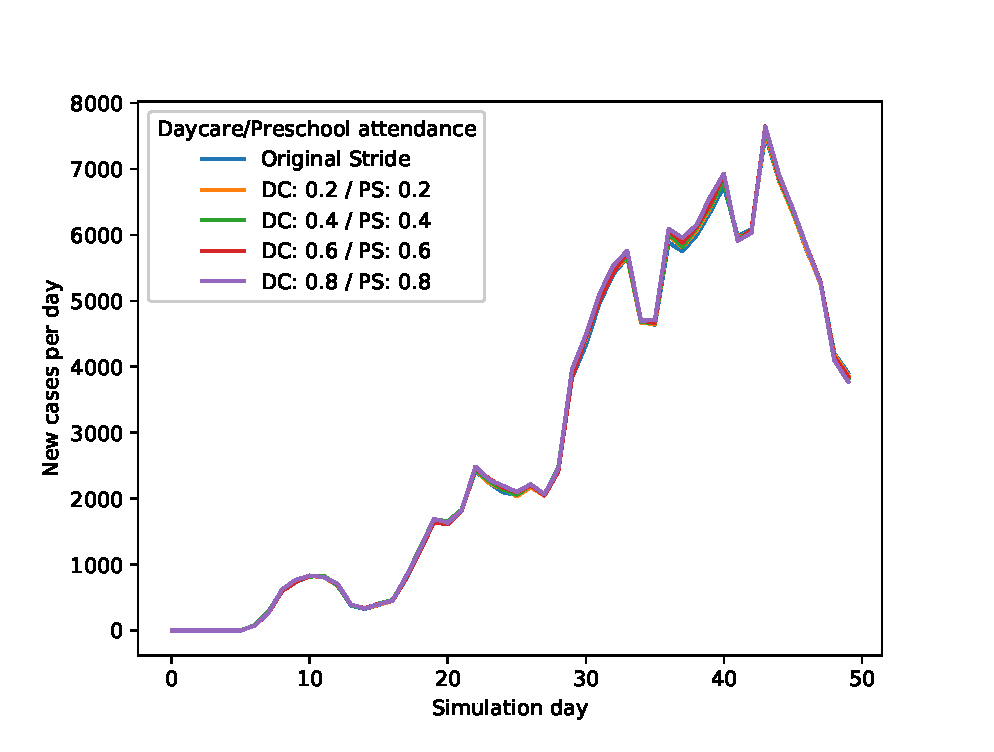
\includegraphics[width=\linewidth]{Daycare-Preschool/cases_per_day_20runs.eps}
		\caption{Average new cases per day.}
	\end{subfigure}
	\begin{subfigure}[b]{0.6\linewidth}
		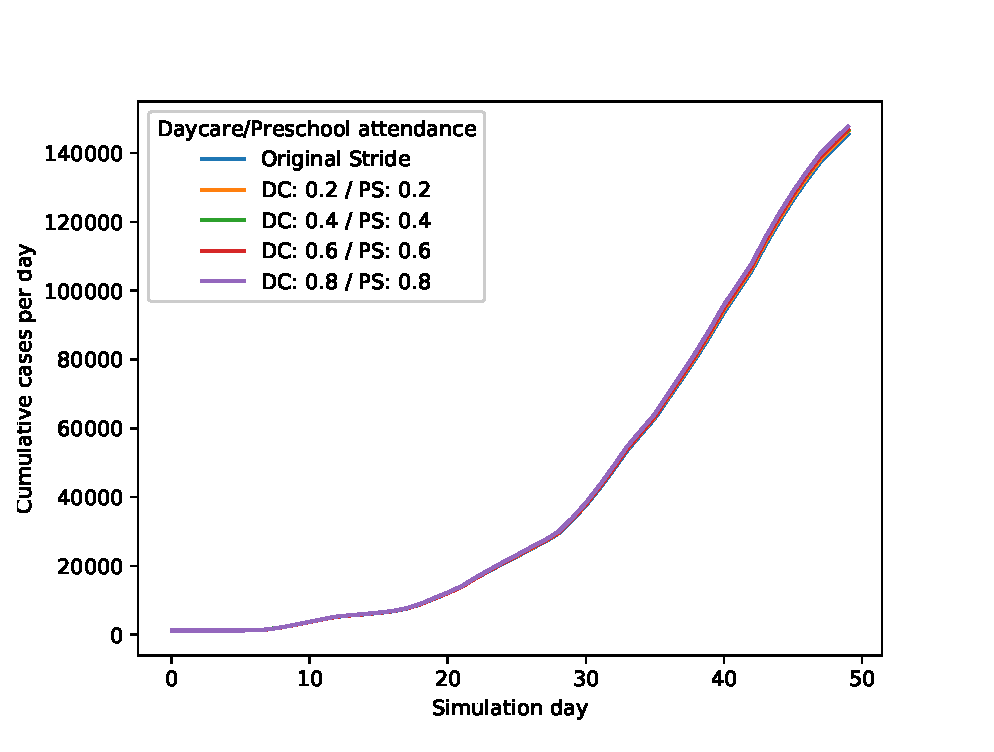
\includegraphics[width=\linewidth]{Daycare-Preschool/cumulative_cases_20runs.eps}
		\caption{Average cumulative cases.}
	\end{subfigure}
	\caption{Simulation results using different degrees of Daycare/Preschool attendance. Averages over 20 runs, seeding rate = 0.2\%, immunity rate = 70\%, $R_0$ = 15. Simulated for a population of 600,000 over 50 days.}
	\label{daycare-preschool}
\end{figure}


\section{Demographic profile}
\paragraph{}
The simulator originally only makes use of one household sample. When doing simulations for Flanders, each province and city will have the same ratio of young to old people. This is not indicative of the real ratio in each of these locations.

The algorithm for creating populations is expanded to allow the use of different household samples. Sample files have to be defined for each province, whereas they are not mandatory for the cities. When for a given city, there is no existing household sample file the algorithm will use the file defined for the entire province.

The simulations here have been done using different demographic profiles. The first profile is represents the original algorithm where only one sample file is used. The second profile uses a sample file for each province in Flanders and a file for each city that is defined as a \emph{centrumstad}.
These cities are ones with a relatively large population compared to their surroundings with a central function in the area of employment, care, education, culture and entertainment.


\begin{figure}[h!]
	\centering
	\begin{subfigure}[b]{0.6\linewidth}
		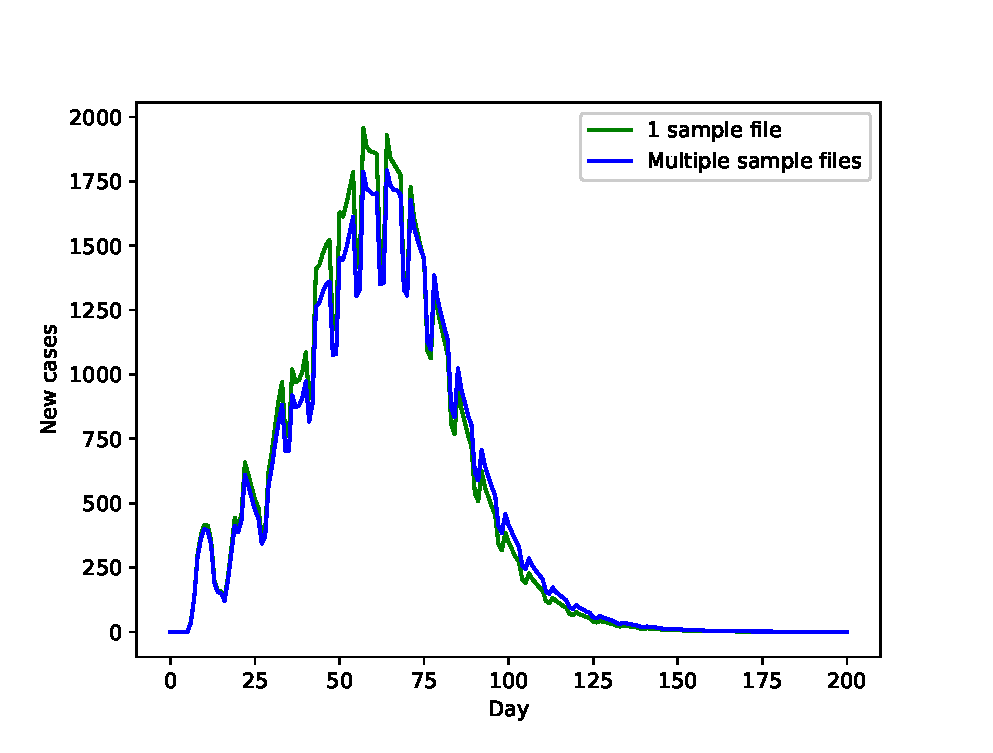
\includegraphics[width=\linewidth]{Demographic/figs/plot_compSize_CASE_PER_DAY_AVG.eps}
		\caption{Average new cases per day.}
	\end{subfigure}
	\begin{subfigure}[b]{0.6\linewidth}
		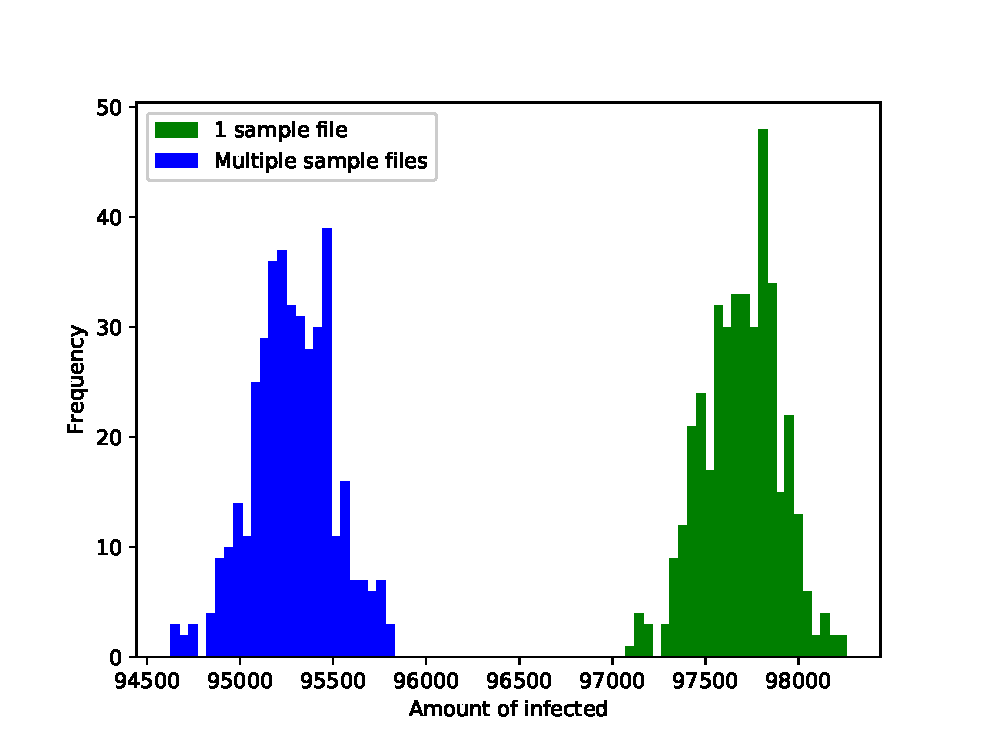
\includegraphics[width=\linewidth]{Demographic/figs/plot_compSize_FINALDAY_HIST.eps}
		\caption{Amount of infected people at the end of the simulation.}
	\end{subfigure}
	\caption{Results of 400 different simulations for the 2 different demographic profiles. Seeding rate = $0.2\%$, immunity rate = $80\%$, $R_0$ = 11. Simulated for a population of 600,000 over 200 days.}
	\label{demographic_profile}
\end{figure}

By visually inspecting figure \ref{demographic_profile} we can see a clear difference in the amount of infected people at the end of the simulation. The outbreaks are larger when using only 1 sample file.

We determined a 95\% confidence interval for the outbreak size for the demographic coming from 1 file:
\[[97673.912, 97714.508]\]

And for the demographic coming from multiple files:
\[[95258.962, 95302.443]\]

These intervals are disjoint and lie apart quite significantly, we can conclude that using multiple household samples instead of only one has an impact on the simulation results.

\section{Workplace Size Distribution}
\paragraph{}
With the addition of the third feature, we can specify different ranges of sizes for workplaces. This means we can have 70\% of workplaces that have a size between 20 and 50 and 30\% between 50 and 100.

The workplace size distribution used in the new algorithm as the default case is the following:
\begin{table}[!h]
	\centering
	\begin{tabular}{|c|c|c|}
		\hline
		Ratio & Minimum size & Maximum size \\\hline
		77.854\% & 1 & 9 \\\hline
		17.190\% & 10 & 49 \\\hline
		4.100\% & 50 & 199 \\\hline
		0.856\% & 200 & 400 \\\hline
	\end{tabular}
\end{table}

while in the original algorithm, all the workplaces are around 20 people large.

To determine whether different size classes in the workplaces have a significant impact on the simulations, the influenza virus is used.
Here, more interesting results, meaning there is a noticeable difference in simulation results, can be seen when the immunity rate is sufficiently low. For this reason we used an immunity rate of 40\%, this means that 60\% of the population can get infected by the influenza virus.
The new algorithm is compared to different sizes of workplaces using the different algorithm, with size 17 being the average for the values used in the new algorithm.

\begin{figure}[h!]
	\centering
	\begin{subfigure}[b]{0.6\linewidth}
		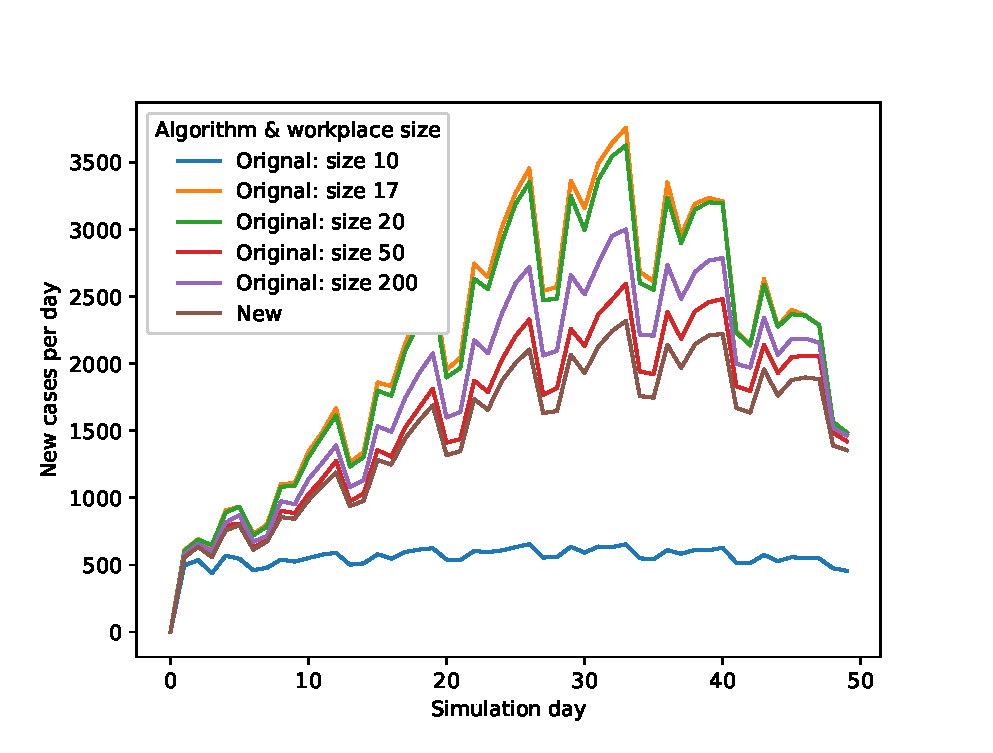
\includegraphics[width=\linewidth]{Workplace/workplace_sizes_ncpd.eps}
		\caption{Average new cases per day.}
	\end{subfigure}
	\begin{subfigure}[b]{0.6\linewidth}
		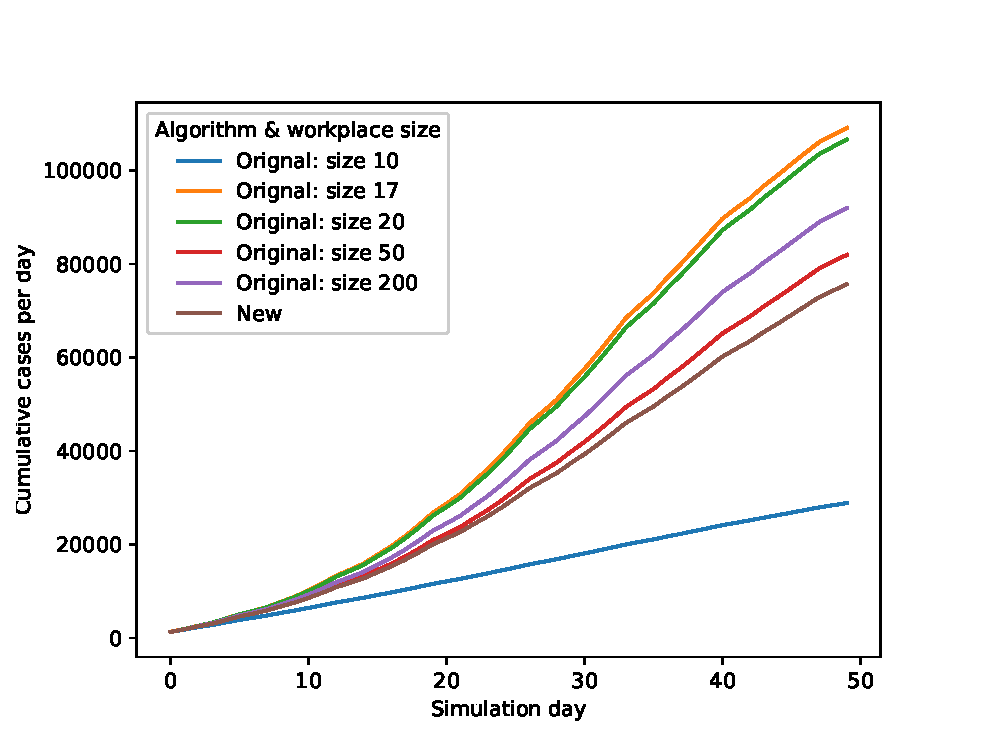
\includegraphics[width=\linewidth]{Workplace/workplace_sizes_ccpd.eps}
		\caption{Average cumulative cases.}
	\end{subfigure}
	\caption{Results of 20 different simulations for varying workplace sizes. Seeding rate = $0.2\%$, immunity rate = $40\%$, $R_0$ = 2. Simulated for a population of 600,000 over 50 days.}
	\label{workplace_immunity}
\end{figure}

The most noticeable result is how a decreasing workplace size leads to more new cases per day, this happens until around size 10 where the amount of new cases drops significantly. Very small workplaces do not allow the disease to spread quickly when compared to the larger ones. A possible explanation here is that the chance to meet an infected person in these workplaces is small.

The average size of workplaces in the new algorithm does not seem to be an important factor.

While running a simulation using the original algorithm and having results of the new algorithm seems possible, finding the correct size of the workplaces is difficult. Each different size of the workplace has their own impact on the spread of the disease, so we can conclude that a combination of those sizes result in a more realistic spread.

\end{document}
